\chapter{System Design Development}

\section{Introduction}

This chapter presents the design development of the HMI Stars system. It describes how the solution was structured and specified using the Unified Process, covering the Inception, Elaboration, and Construction phases.
It details the functional analysis through use case modeling, followed by system design using UML diagrams, architectural decisions, and class modeling. It also presents the transition from logical design to implementation, including database mapping, system modularization, and deployment choices.

\section{Phase of Inception}

During the Inception phase, the development process separates into two parallel tracks following the 2TUP methodology. The \textbf{Functional Track} focuses on eliciting user requirements, modeling use cases, and drafting user interface prototypes to define the system's behavioral scope. Concurrently, the \textbf{Technical Track} analyzes initial technology constraints (such as selecting Flutter and Supabase, as detailed in Chapter 1) to prepare the architectural foundations. The subsections below detail the activities and deliverables of the Functional Track for this phase.

\subsection{Use Case Model Development}
During the inception phase, we defined the system actors and their corresponding use cases. Since the solution is composed of two distinct interfaces: a mobile application and a web application: both connected to a shared database, the functional requirements were represented using three use case diagrams: a general system overview, a mobile-oriented diagram, and a web-oriented diagram.


\subsubsection{Global Use Case Diagram}
Figure 2.1 presents the global use case diagram, showing how the Client and HMI Stars Manager interact with the overall ecosystem.
\begin{figure}[H]
    \centering
    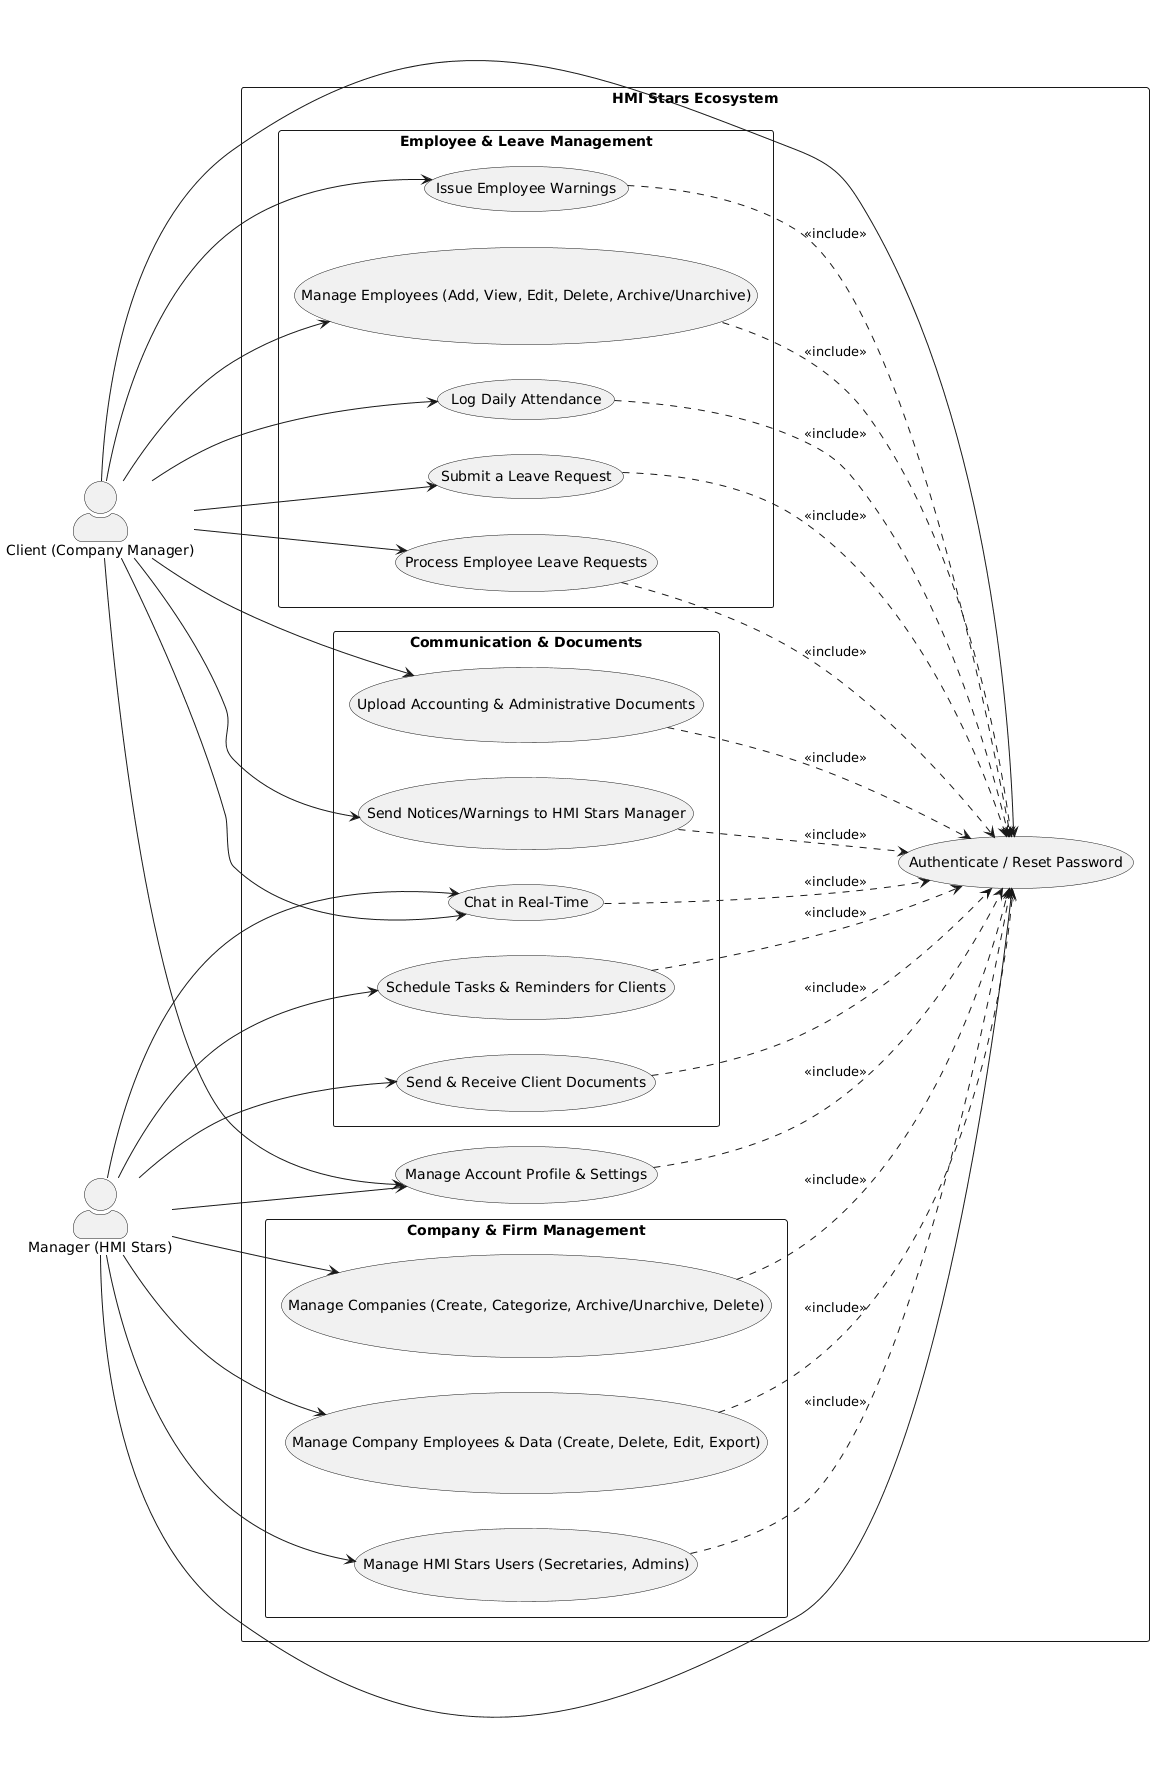
\includegraphics[width=0.95\textwidth]{diagrams/usecase.png}
    \caption{Global Use Case Diagram}
    \label{fig:use_case_design}
\end{figure}

\subsubsection{Mobile Client Application Use Case Diagram}
Figure 2.2 illustrates the functional scope of the mobile application dedicated to client company managers, focusing on personnel tracking, pointage logging, leave requests, document uploads, and real-time chat.
\begin{figure}[H]
    \centering
    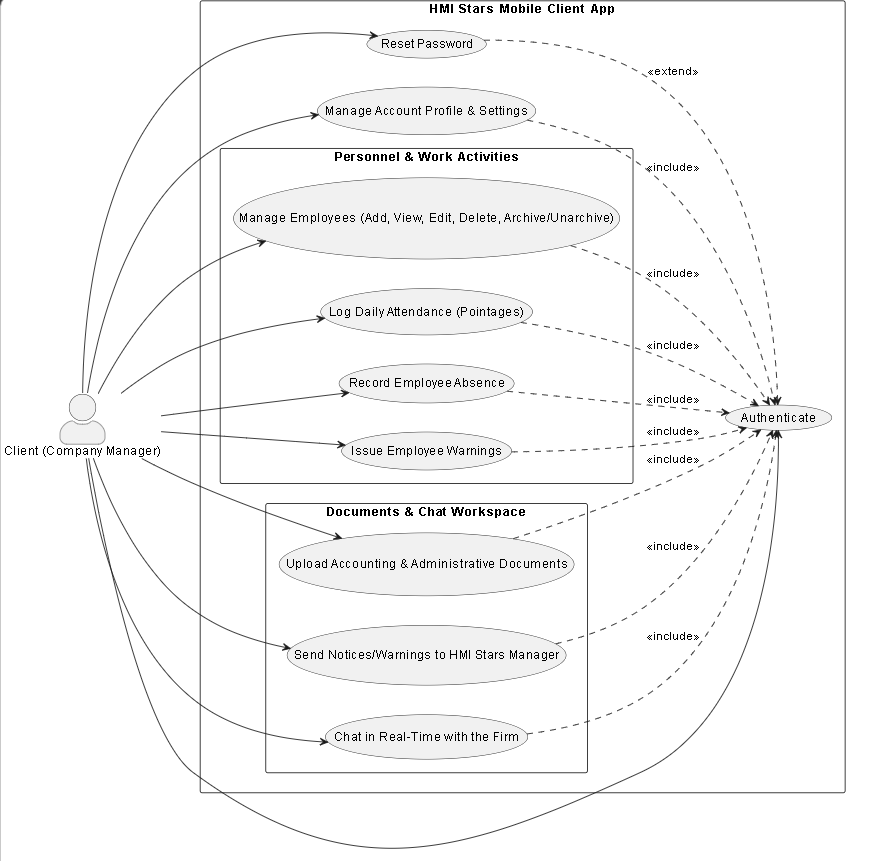
\includegraphics[width=0.9\textwidth]{diagrams/app_usecase.png}
    \caption{Mobile Application Use Case Diagram}
    \label{fig:use_case_mobile}
\end{figure}

\subsubsection{web application Use Case Diagram}
Figure 2.3 shows the functional scope of the web application used by HMI Stars managers and administrative staff. \\
It focuses on client company registration, employee record access, data export, task scheduling, role management, and real-time messaging.

\begin{figure}[H]
    \centering
    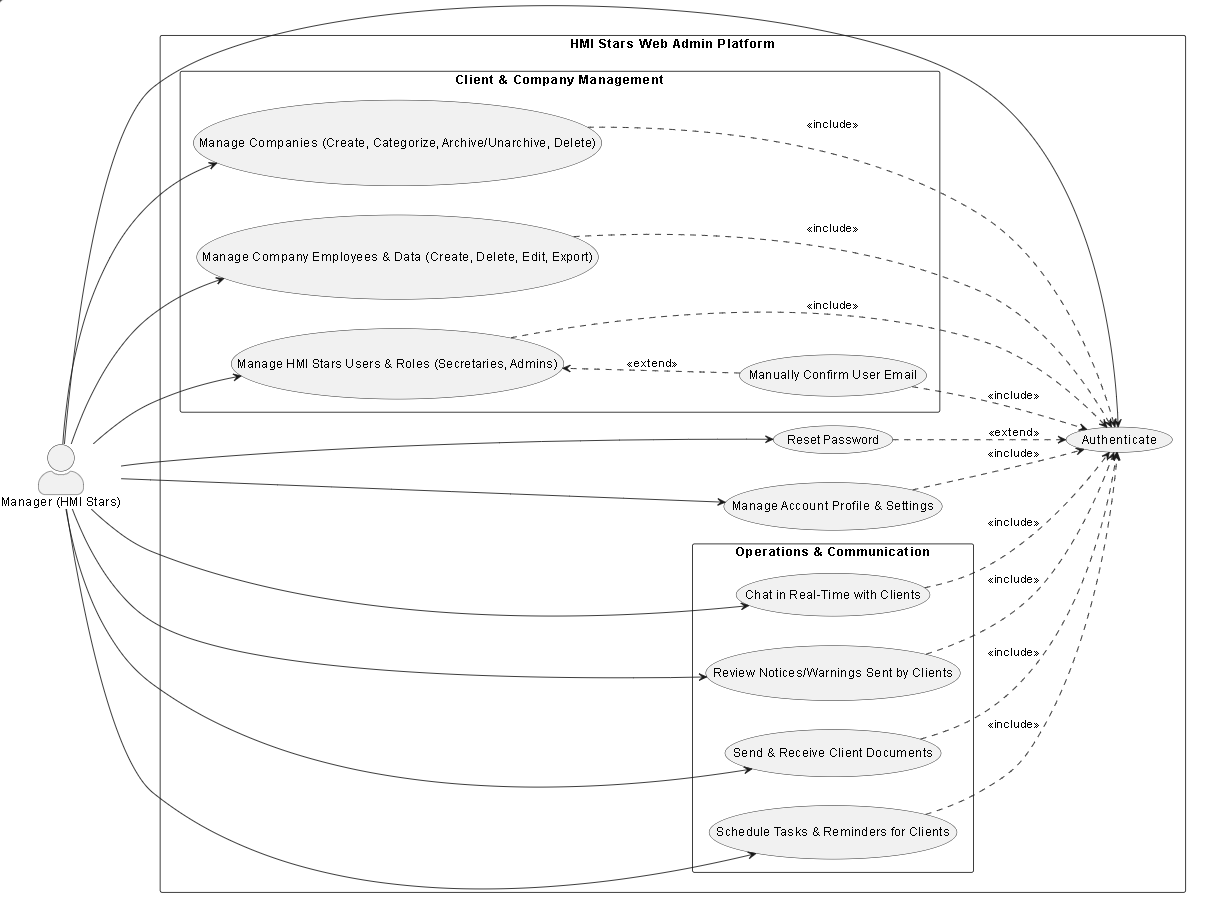
\includegraphics[width=0.9\textwidth]{diagrams/platform_usecase.png}
    \caption{WebApp Use Case Diagram}
    \label{fig:use_case_web}
\end{figure}

\subsection{Definition of Priorities}
To plan the construction phase, functional use cases were prioritized based on business value and technical risk, as shown in Table 2.1.

\begin{table}[H]
\centering
\caption{Priority assignment table}
\label{tab:priorities}
\begin{tabular}{|l|l|l|l|}
\hline
\textbf{Use Case} & \textbf{Priority} & \textbf{Complexity} & \textbf{Target Iteration} \\
\hline
UC-01: Authenticate & High & Medium & Iteration 1 \\
\hline
UC-02: Manage Employees & High & Medium & Iteration 1 \\
\hline
UC-03: Submit Attendance (Pointage) & High & High & Iteration 2 \\
\hline
UC-04: Submit Leave Request & Medium & Medium & Iteration 2 \\
\hline
UC-05: Real-time Chat & High & High & Iteration 3 \\
\hline
UC-06: Upload Documents & High & Low & Iteration 3 \\
\hline
UC-07: Manage Warnings \& Templates & Medium & Medium & Iteration 4 \\
\hline
UC-08: Settings \& Personalization & Low & Low & Iteration 4 \\
\hline
UC-09: Document Scanner & Medium & High & Iteration 4 \\
\hline
\end{tabular}
\end{table}

\subsection{Detailed Description of Use Cases}
The following tables provide the formal textual description for each prioritized use case identified in Table \ref{tab:priorities}.

\begin{table}[H]
\centering
\caption{UC-01: Authenticate}
\label{tab:uc01}
\begin{tabular}{|l|p{10cm}|}
\hline
\textbf{Actor} & Client (Mobile) / HMI Manager (Web) \\
\hline
\textbf{Precondition} & The user has a registered account with valid credentials. \\
\hline
\textbf{Main Flow} & 1. The user opens the login screen.\newline 2. The user enters their email and password.\newline 3. The system validates the credentials against Supabase Auth.\newline 4. The system redirects the user to the dashboard. \\
\hline
\textbf{Alternative Flow} & If credentials are invalid, the system displays an error message and remains on the login screen. \\
\hline
\textbf{Postcondition} & The user is authenticated and has access to their role-based dashboard. \\
\hline
\end{tabular}
\end{table}

\begin{table}[H]
\centering
\caption{UC-02: Manage Employees}
\label{tab:uc02}
\begin{tabular}{|l|p{10cm}|}
\hline
\textbf{Actor} & Client (Mobile \& Web) \\
\hline
\textbf{Precondition} & The client is authenticated and has a registered company. \\
\hline
\textbf{Main Flow} & 1. The client navigates to the employees section.\newline 2. The client adds a new employee by filling in personal and contract details.\newline 3. The system stores the employee record in the database.\newline 4. The employee appears in the active registry list. \\
\hline
\textbf{Alternative Flow} & The client can also edit existing employee information or archive an inactive employee. \\
\hline
\textbf{Postcondition} & The employee record is created, updated, or archived in the database. \\
\hline
\end{tabular}
\end{table}

\begin{table}[H]
\centering
\caption{UC-03: Submit Attendance (Pointage)}
\label{tab:uc03}
\begin{tabular}{|l|p{10cm}|}
\hline
\textbf{Actor} & Client (Mobile) \\
\hline
\textbf{Precondition} & The client is authenticated and has active employees registered under their company. \\
\hline
\textbf{Main Flow} & 1. The client navigates to the ``Pointage'' section.\newline 2. The system loads the list of active employees.\newline 3. The client selects a date from the calendar.\newline 4. The client marks the attendance status (present/absent) for each employee.\newline 5. The client clicks ``Save''.\newline 6. The system records the attendance in the PostgreSQL database. \\
\hline
\textbf{Alternative Flow} & If the network is unavailable, the system caches the records locally and synchronizes them once connection is restored. \\
\hline
\textbf{Postcondition} & Daily attendance records are saved and visible in the attendance history. \\
\hline
\end{tabular}
\end{table}

\begin{table}[H]
\centering
\caption{UC-04: Submit Leave Request}
\label{tab:uc04}
\begin{tabular}{|l|p{10cm}|}
\hline
\textbf{Actor} & Client (Mobile) \\
\hline
\textbf{Precondition} & The client is authenticated and has active employees. \\
\hline
\textbf{Main Flow} & 1. The client navigates to the leave request section.\newline 2. The client selects an employee, a leave type, and start/end dates.\newline 3. The client optionally adds a comment and submits the request.\newline 4. The system stores the leave entry in the database. \\
\hline
\textbf{Alternative Flow} & If required fields are missing, the system displays a validation error and prevents submission. \\
\hline
\textbf{Postcondition} & The leave request is recorded and appears in the leave history list. \\
\hline
\end{tabular}
\end{table}

\begin{table}[H]
\centering
\caption{UC-05: Real-Time Chat}
\label{tab:uc05}
\begin{tabular}{|l|p{10cm}|}
\hline
\textbf{Actor} & Client (Mobile) / HMI Manager (Web) \\
\hline
\textbf{Precondition} & Both the client and the HMI manager are authenticated. \\
\hline
\textbf{Main Flow} & 1. The user opens the messaging section.\newline 2. The user selects a conversation.\newline 3. The user types and sends a message.\newline 4. The system transmits the message via Supabase real-time WebSocket.\newline 5. The message appears instantly on both sides. \\
\hline
\textbf{Alternative Flow} & The user can attach a file or image instead of text. The system uploads the file to Supabase Storage and shares the download link in the conversation. \\
\hline
\textbf{Postcondition} & The message is stored in the database and visible to both participants. \\
\hline
\end{tabular}
\end{table}

\begin{table}[H]
\centering
\caption{UC-06: Upload Documents}
\label{tab:uc06}
\begin{tabular}{|l|p{10cm}|}
\hline
\textbf{Actor} & Client (Mobile) / HMI Manager (Web) \\
\hline
\textbf{Precondition} & The user is authenticated and associated with a company. \\
\hline
\textbf{Main Flow} & 1. The user navigates to the documents section.\newline 2. The user selects a document category (KBIS, VAT, RIB, etc.).\newline 3. The user uploads a file from the device.\newline 4. The system stores the file in Supabase Storage and creates a metadata record. \\
\hline
\textbf{Alternative Flow} & If the file exceeds the size limit or has an unsupported format, the system rejects the upload with an error message. \\
\hline
\textbf{Postcondition} & The document is stored and visible in the company's document list. \\
\hline
\end{tabular}
\end{table}

\begin{table}[H]
\centering
\caption{UC-07: Manage Warnings \& Templates}
\label{tab:uc07}
\begin{tabular}{|l|p{10cm}|}
\hline
\textbf{Actor} & HMI Manager (Web) / Client (Mobile) \\
\hline
\textbf{Precondition} & The user is authenticated. Warning letter templates exist in the system. \\
\hline
\textbf{Main Flow} & 1. The user navigates to the warnings section.\newline 2. The user selects or creates a warning template.\newline 3. The user fills in the employee name, date, and reason.\newline 4. The user sends the letter via Gmail integration. \\
\hline
\textbf{Alternative Flow} & The user can save a draft template for future reuse without sending. \\
\hline
\textbf{Postcondition} & The warning letter is generated and sent, or the template is saved for later use. \\
\hline
\end{tabular}
\end{table}

\begin{table}[H]
\centering
\caption{UC-08: Settings \& Personalization}
\label{tab:uc08}
\begin{tabular}{|l|p{10cm}|}
\hline
\textbf{Actor} & Client (Mobile) / HMI Manager (Web) \\
\hline
\textbf{Precondition} & The user is authenticated. \\
\hline
\textbf{Main Flow} & 1. The user opens the settings screen.\newline 2. The user changes preferences such as language (FR/EN) or theme (Light/Dark).\newline 3. The system applies the changes immediately and stores the preferences. \\
\hline
\textbf{Alternative Flow} & The user can also update profile information (name, avatar). \\
\hline
\textbf{Postcondition} & The user's preferences are persisted and applied across all sessions. \\
\hline
\end{tabular}
\end{table}

\begin{table}[H]
\centering
\caption{UC-09: Document Scanner}
\label{tab:uc09}
\begin{tabular}{|l|p{10cm}|}
\hline
\textbf{Actor} & Client (Mobile) \\
\hline
\textbf{Precondition} & The client is authenticated and camera permission is granted. \\
\hline
\textbf{Main Flow} & 1. The client opens the scanner from the chat or documents section.\newline 2. The client captures a photo of a physical document.\newline 3. The system applies cropping and contrast filters.\newline 4. The client confirms and sends the scanned image as an attachment. \\
\hline
\textbf{Alternative Flow} & The client can retake the photo or adjust the crop before confirming. \\
\hline
\textbf{Postcondition} & The scanned document image is uploaded and attached to the conversation or document list. \\
\hline
\end{tabular}
\end{table}


\subsection{User Interface Prototypes}
To validate the initial user flows and interaction concepts before starting implementation, we drafted low-fidelity interface mockups. We focused on designing structured dashboards for both client-side and administration-side interfaces to coordinate information access.

Figure \ref{fig:mobile_wireframe} presents the mobile dashboard interface mockup, detailing the top welcome header, the key human resource metric cards, and the warning alert notification area. Figure \ref{fig:web_wireframe} illustrates the web administration portal dashboard prototype, highlighting the sidebar navigation on the left, top menu bar controls, and the central analytics charts workspace on the right.

\begin{figure}[H]
    \centering
    \begin{subfigure}[b]{0.45\textwidth}
        \centering
        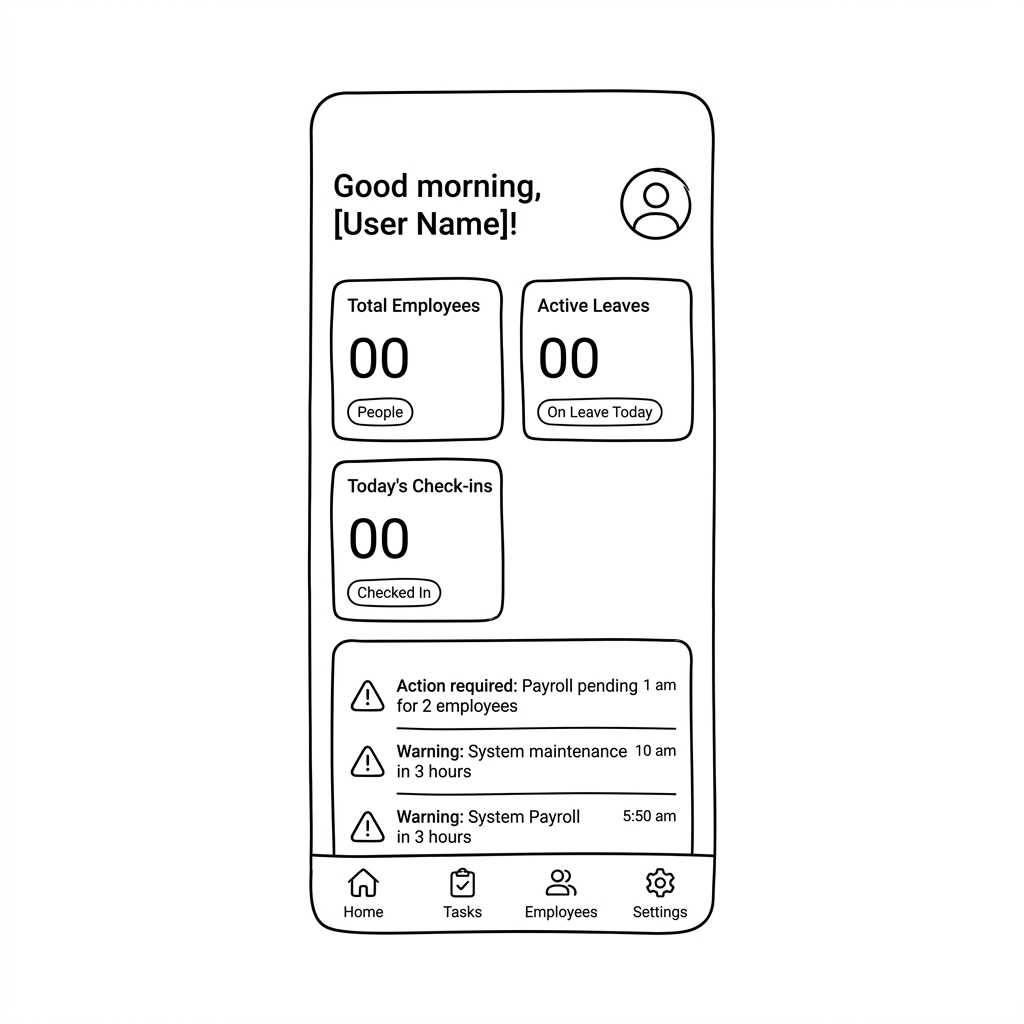
\includegraphics[width=1.2\textwidth]{images/mobile_attendance_wireframe.png}
        \caption{Mobile Dashboard Wireframe}
        \label{fig:mobile_wireframe}
    \end{subfigure}
    \hfill
    \begin{subfigure}[b]{0.45\textwidth}
        \centering
        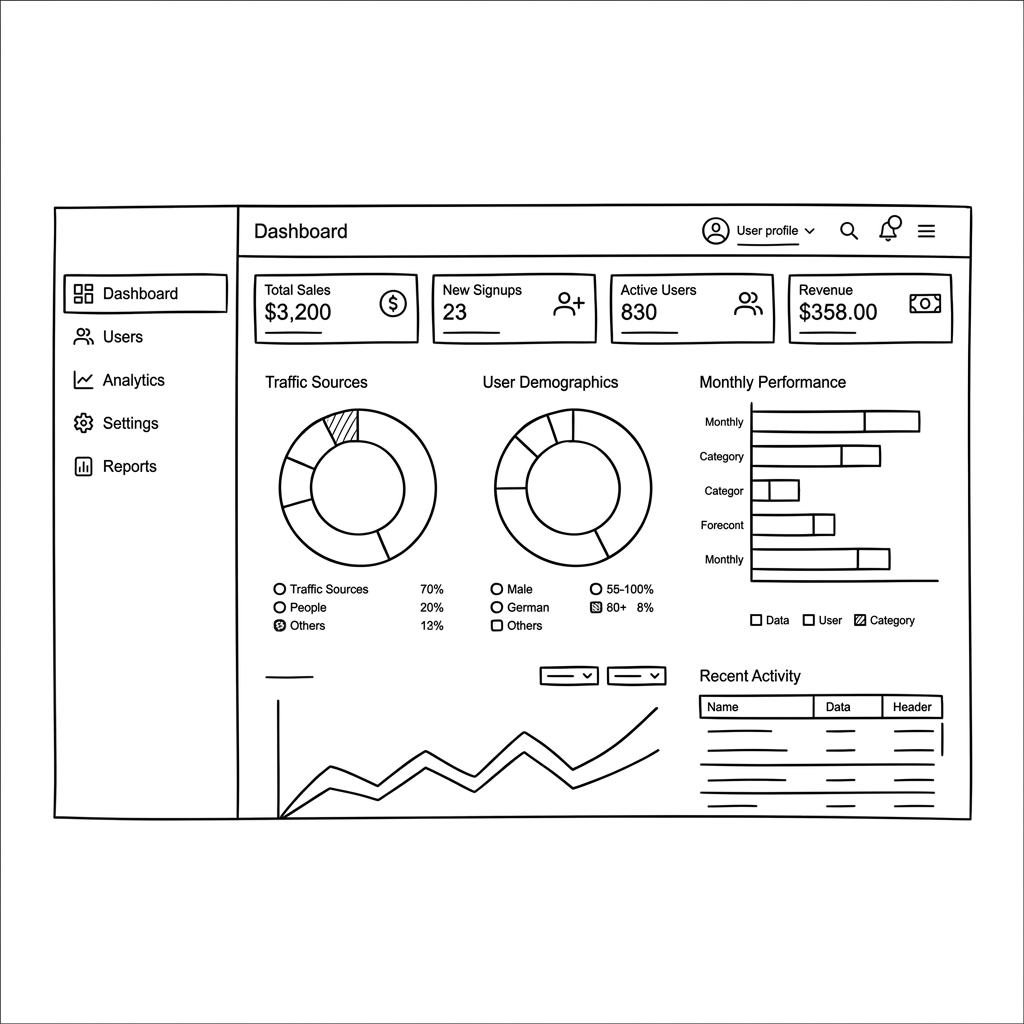
\includegraphics[width=\textwidth]{images/web_dashboard_wireframe.png}
        \caption{Web Dashboard Workspace Wireframe}
        \label{fig:web_wireframe}
    \end{subfigure}
    \caption{Low-Fidelity User Interface Prototypes}
    \label{fig:ui_wireframes}
\end{figure}

\section{Phase of Elaboration}

The Elaboration phase represents the parallel progression and refinement of both tracks. The \textbf{Technical Track} establishes the system's non-functional parameters, architectural style, and overall deployment topology (see Subsections \ref{subsec:arch_analysis} and \ref{subsec:arch_design}). Simultaneously, the \textbf{Functional Track} focuses on detailing dynamic behavior and class relationships through sequence diagrams and class diagrams (see Subsections \ref{subsec:uc_analysis} and \ref{subsec:uc_design}). This dual approach ensures that the functional requirements are fully supported by a robust, secure technical framework.

\subsection{Architectural Analysis}
\label{subsec:arch_analysis}
During the elaboration phase, we analyzed the structural constraints that shape the system architecture. The HMI Stars ecosystem must support cross-platform mobile and web-based administration while ensuring strict database-level data isolation between client companies.

\subsubsection{Non-Functional Requirements}
Table \ref{tab:nfr} identifies the key non-functional requirements that guided the architectural decisions.

\begin{table}[H]
\centering
\caption{Non-functional requirements}
\label{tab:nfr}
\begin{tabular}{|l|p{9.5cm}|}
\hline
\textbf{Requirement} & \textbf{Description} \\
\hline
\textbf{Security} & Each client company must access only its own data. Row Level Security (RLS) policies enforce per-company isolation directly at the PostgreSQL level. \\
\hline
\textbf{Real-time responsiveness} & Chat messages, file uploads, and attendance updates must propagate to all connected clients within seconds via WebSocket channels. \\
\hline
\textbf{Cross-platform compatibility} & The solution must run on Android devices (mobile app) and modern web browsers (admin platform) from a single codebase. \\
\hline
\textbf{Availability} & The backend must remain accessible at all times. Supabase provides managed cloud hosting with automated backups and failover. \\
\hline
\textbf{Offline tolerance} & The mobile application must allow attendance logging even without network connectivity, with automatic synchronization upon reconnection. \\
\hline
\textbf{Maintainability} & The codebase must follow a modular structure so that new features (e.g., payroll, contracts) can be added without modifying existing modules. \\
\hline
\end{tabular}
\end{table}

\subsubsection{Architectural Style}
We adopted a \textbf{client-server architecture} with a shared Backend-as-a-Service (BaaS) layer. In this approach, both the mobile application and the web platform act as independent frontend clients that communicate with a centralized Supabase backend through REST API calls and real-time WebSocket subscriptions.

We considered two alternative architectural approaches before selecting this model:
\begin{itemize}
    \item \textbf{Custom REST API (Node.js / Express):} This approach would require building and maintaining a dedicated backend server, handling authentication, session management, and API routing manually. We rejected it because the project scope did not justify the added infrastructure complexity, and Supabase provides all required services (auth, database, storage, real-time) out of the box.
    \item \textbf{Microservices architecture:} Splitting the backend into independent services (auth service, chat service, document service) would improve scalability but introduce significant operational overhead (service discovery, inter-service communication, deployment orchestration). Given the small team size and the consulting firm's user volume, this level of distribution was unnecessary.
\end{itemize}

The chosen BaaS architecture offers several advantages for this project: zero server-side code for standard CRUD operations, built-in authentication with email/OTP support, native PostgreSQL RLS for data isolation, and a managed real-time engine — all reducing development time while maintaining production-grade security.


\subsection{Use Case Analysis}
\label{subsec:uc_analysis}
We model the dynamic interactions of use cases using UML sequence diagrams to show the workflow between frontend components, the routing system, the database tables, and actors.

\subsubsection{Password Recovery \& Authentication Sequence}
The sequence diagram in Figure \ref{fig:sequence_auth_design} details the password recovery process.\\ It highlights how the Flutter Router handles the URL hash parameters to initialize a session directly from the Supabase redirect link without requiring credentials manually.
\begin{figure}[H]
    \centering
    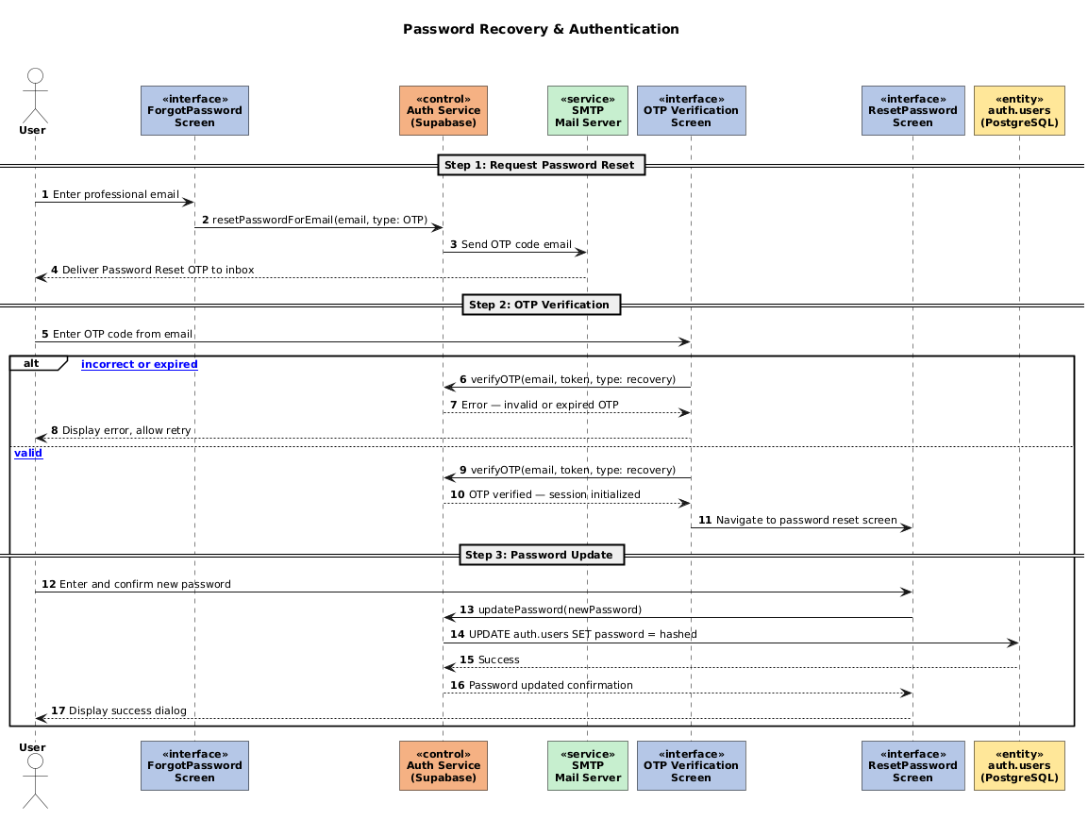
\includegraphics[width=1\textwidth]{diagrams/auth_sequence_diagram.png}
    \caption{Authentication Sequence Diagram - Password Recovery}
    \label{fig:sequence_auth_design}
\end{figure}

\subsubsection{Leave Request Submission Sequence}
Figure \ref{fig:sequence_leave_design} shows the sequence of submitting a leave request, highlighting how the Client submits it, how Row Level Security policies validate the transaction, and how it is registered in the database.
\begin{figure}[H]
    \centering
    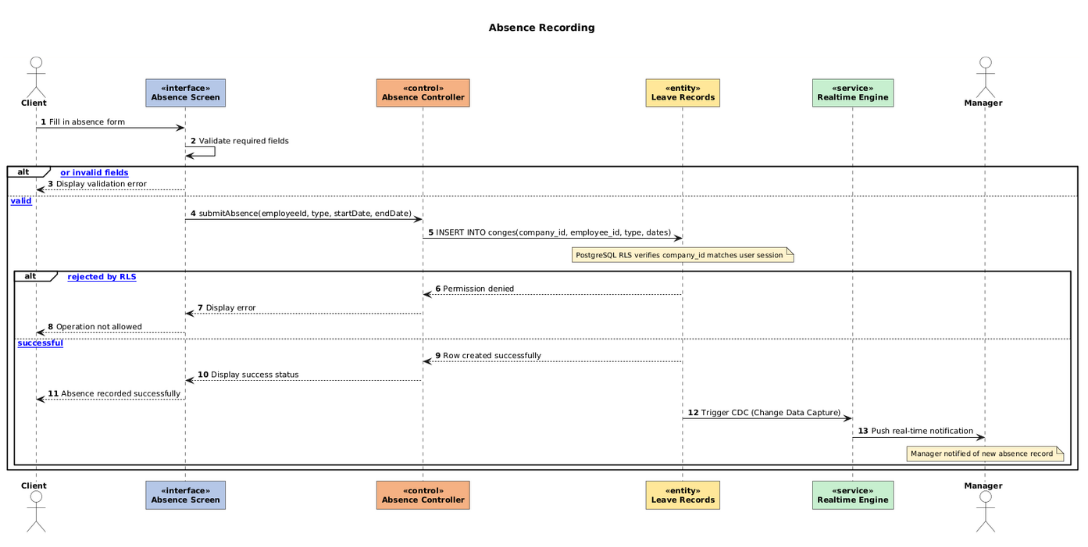
\includegraphics[width=1\textwidth]{diagrams/leave_sequence_diagram.png}
    \caption{Sequence Diagram - Leave Request Submission Flow}
    \label{fig:sequence_leave_design}
\end{figure}

\subsubsection{Real-time Messaging Sequence}
Figure \ref{fig:sequence_chat_design} illustrates the instant communication sequence. It displays how PostgreSQL write operations are instantly pushed to listeners via Supabase's Realtime WebSocket engine to keep the client mobile application and web application synchronized.
\begin{figure}[H]
    \centering
    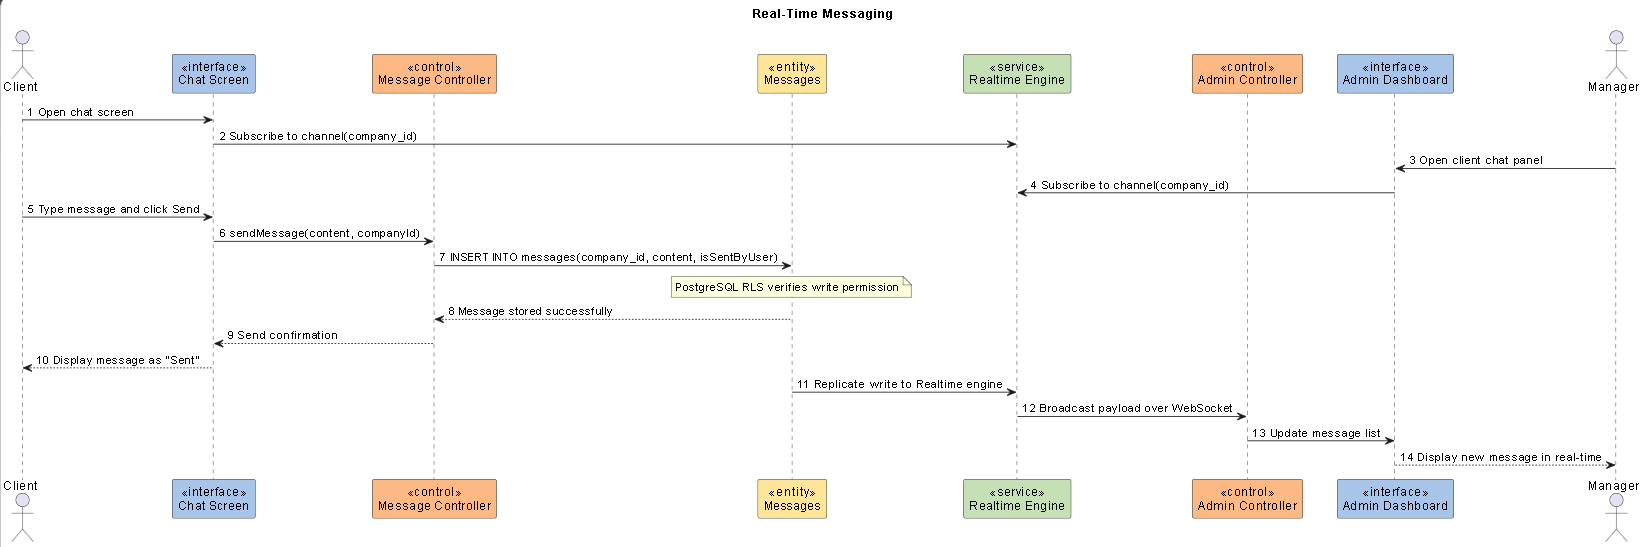
\includegraphics[width=1\textwidth]{diagrams/chat_sequence_diagram.png}
    \caption{Sequence Diagram - Real-Time Message Sync Flow}
    \label{fig:sequence_chat_design}
\end{figure}

\subsubsection{Dual-OTP Email Modification Sequence}
To secure client manager accounts from unauthorized takeover during email updates, a dual-OTP verification sequence is executed. Figure \ref{fig:sequence_dual_otp} details this flow, showing how both the old and new email addresses must be verified sequentially using native in-app OTP entry.

\begin{figure}[H]
    \centering
    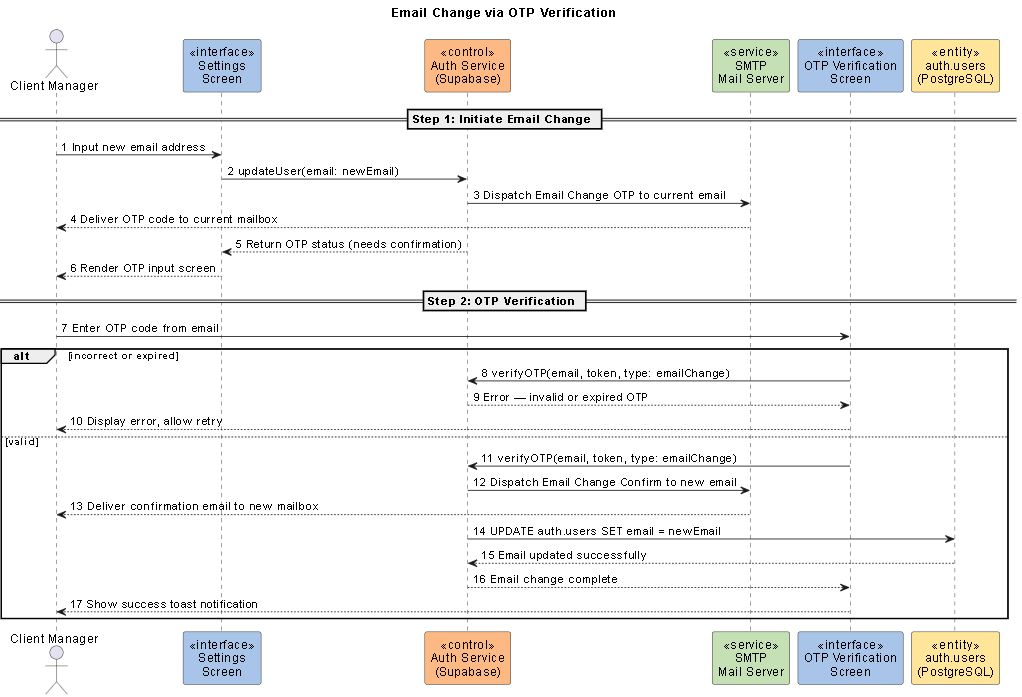
\includegraphics[width=1\textwidth]{diagrams/otp_sequence_diagram.png}
    \caption{Sequence Diagram - Dual-OTP Email Modification Flow}
    \label{fig:sequence_dual_otp}
\end{figure}

\subsection{Architectural Design}
\label{subsec:arch_design}
The architectural design defines the subsystems. We adopted a Monorepo client-server pattern. Both client applications (Web and Mobile) communicate with Supabase via REST APIs and WebSockets, as detailed in the system architecture and data flow diagram (Figure \ref{fig:architecture_design}).

\begin{figure}[H]
    \centering
    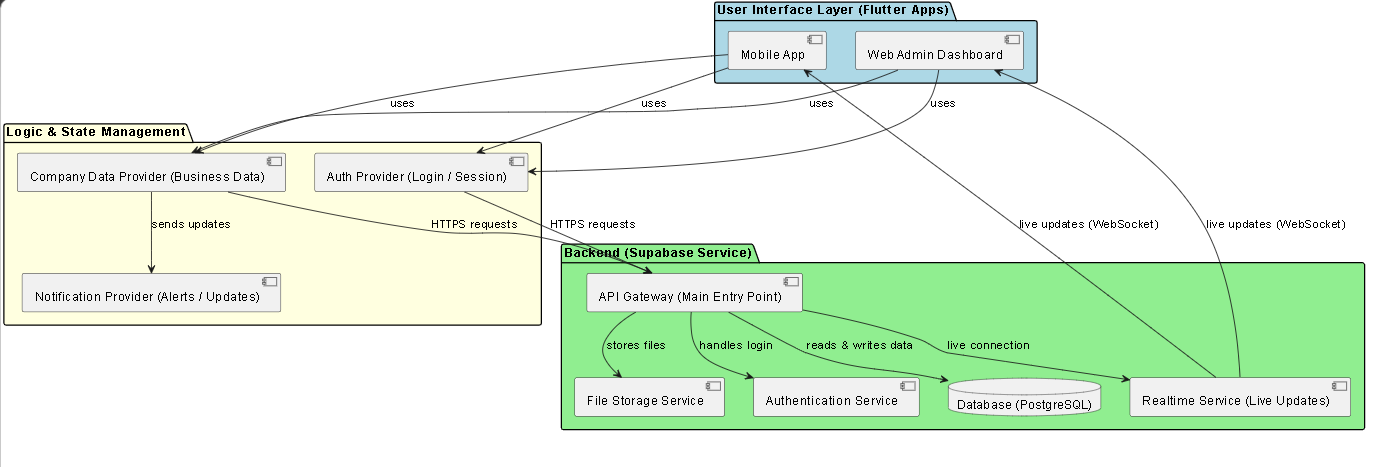
\includegraphics[width=1\textwidth]{diagrams/arch_diagram.png}
    \caption{System Architecture and Data Stream Diagram}
    \label{fig:architecture_design}
\end{figure}

\subsection{Use Case Design}
\label{subsec:uc_design}
The use case design maps objects to the logical class diagram. Figure \ref{fig:class_diag} shows the model class relationships matching the database schema.
\begin{figure}[H]
    \centering
    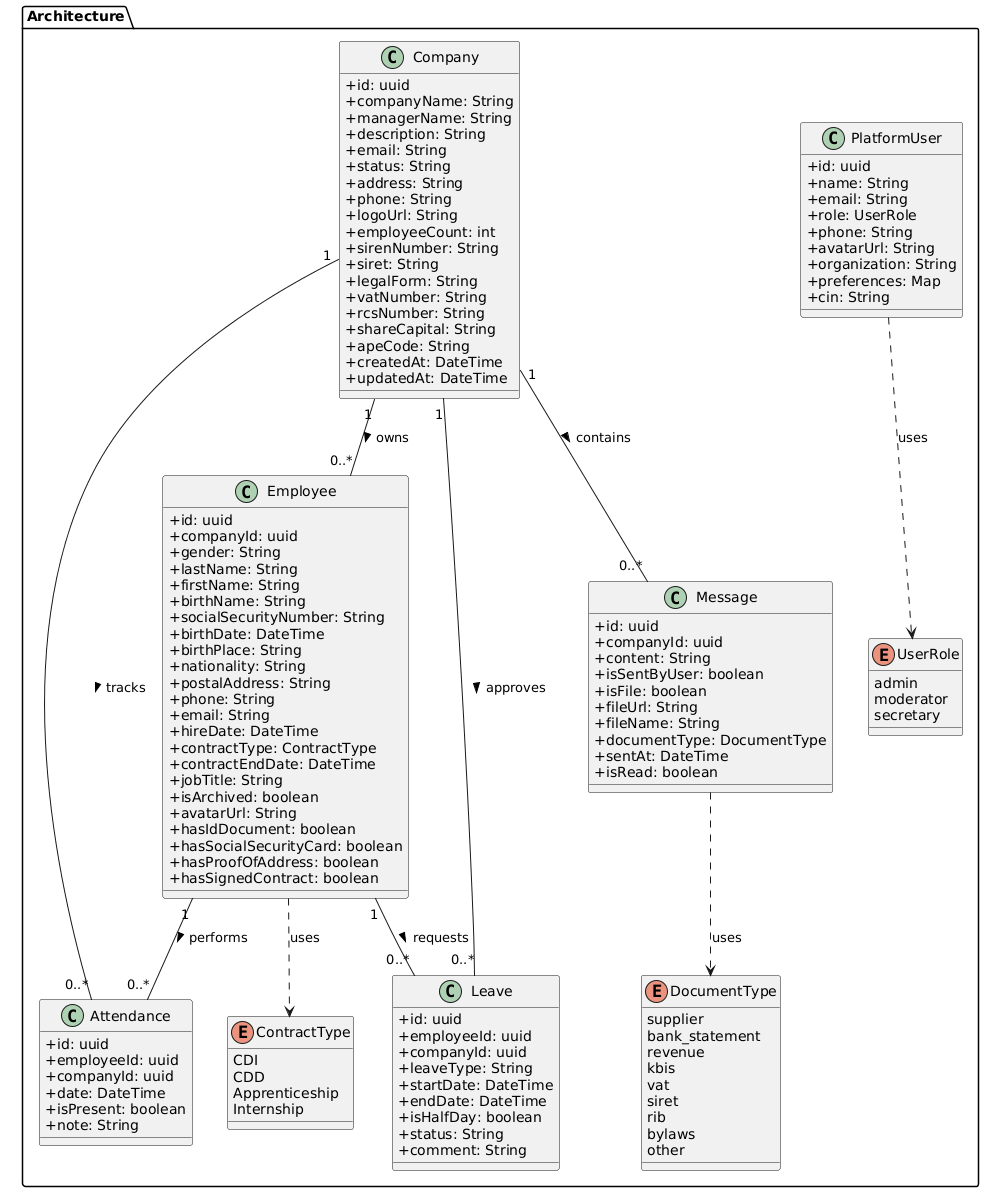
\includegraphics[width=1.01\textwidth]{diagrams/class_diagram.png}
    \caption{Logical Class Diagram of the System}
    \label{fig:class_diag}
\end{figure}
\section{Phase of Construction}

During the Construction phase, the Functional and Technical tracks of the 2TUP methodology converge. The logical models, use case flows, and user interface layouts defined in the Functional Track are systematically mapped onto the physical database schemas, modular code subsystems, and application frameworks established in the Technical Track. The subsections below describe this convergence, detailing how the database tables are physically implemented, how security isolation (RLS) is applied, how subsystems are modularized, and how the use cases are realized.

\subsection{Database Mapping}
The logical classes are mapped to physical PostgreSQL tables.\\
\textbf{entreprises} : Stores client company registration data, legal details (SIRET, SIREN, legal form, capital), contact information, and logo URLs.\\
\textbf{salaries} : Contains employee registry files including personal credentials (social security number, birth details) and contract statuses.\\
\textbf{pointages} : Records daily attendance and check-in logs for registered company employees.\\
\textbf{conges} : Stores leave and absence requests (start/end dates, type of leave, comment, and status).\\
\textbf{messages} : Stores real-time chat messages and file transfers exchanged between HMI managers and company clients.\\
\textbf{fichiers} : Catalogs uploaded administrative and accounting documents (Extrait KBIS, VAT declarations, RIB, bank statements).\\
\textbf{utilisateurs\_plateforme} : Manages profile metadata and roles (Admin, Moderator, Secretary) for HMI Stars platform staff.\\
\textbf{notes\_entreprises} : Contains internal notes, follow-up logs, and specific notes recorded by HMI staff for each client company.\\
\textbf{taches\_urgentes} : Manages scheduled reminders, alerts, and urgent tasks associated with client accounts.\\
\textbf{modeles\_avertissements} : Stores letter templates for warnings, summons, and other formal disciplinary procedures.\\
\textbf{preferences} : Stores individual user preference configurations and notification\\ settings.\\

To enforce complete security isolation, PostgreSQL \textbf{Row Level Security (RLS)}  is enabled on all tables. The client can only read data where the company ID matches their own authenticated organization ID.

\subsection{Implementation Environment}
Table \ref{tab:impl_env} details the tools and platforms used throughout the development and testing of the HMI Stars system.

\begin{table}[H]
\centering
\caption{Development tools and implementation environment}
\label{tab:impl_env}
\begin{tabular}{|l|p{3.5cm}|p{7cm}|}
\hline
\textbf{Category} & \textbf{Tool / Platform} & \textbf{Role} \\
\hline
IDE & Visual Studio Code & Primary code editor with Flutter, Dart, and SQL extensions \\
\hline
Frontend SDK & Flutter SDK (Dart) & Cross-platform UI framework for building the mobile and web applications from a single codebase \\
\hline
Backend & Supabase (Cloud) & Backend-as-a-Service providing PostgreSQL database, authentication, real-time WebSocket engine, and storage \\
\hline
Backend CLI & Supabase CLI & Local database migrations, schema management, and Edge Function deployment \\
\hline
Version Control & Git \& GitHub & Source code versioning and remote repository hosting \\
\hline
Mobile Emulator & Android Studio Emulator & Testing and debugging the mobile APK on virtual Android devices \\
\hline
Web Browser & Microsoft Edge / Chrome & Running and testing the web administration platform locally \\
\hline
\end{tabular}
\end{table}

\subsection{Identification of Implementation Subsystems}
The code is modularized into feature folders following clean architecture guidelines:
\textbf{1. Core Subsystem :} Theme configurations, routing services, and Supabase client helpers.\\
\textbf{2. Auth Feature Subsystem :}  Sign-in, sign-up, and password recovery controllers.
\textbf{3. Client Management Subsystem :} Employees list, attendance forms, and leave requests.\\
\textbf{4. Messaging Subsystem :} Real-time chat widget, WebSocket listeners, and file upload services.

\subsubsection{Design Pattern \& Architectural Layers}
The codebase of both the mobile and web client applications is structured around a \\ decoupled \textbf{Model-View-Controller (MVC)} design pattern to separate business logic from the user interface presentation: \\

\textbf{Model Layer}: Contains Dart entity models mapping our database records. They manage JSON serialization and deserialization (`fromJson`/`toJson` factories). \\
\textbf{View Layer}: Renders UI screens using responsive Flutter widgets. Views observe state changes and rebuild when notified. \\
\textbf{Controller/State Layer (AppState)}: Exposes actions, processes asynchronous transactions, and dispatches data change signals to UI consumers.
\subsection{Deployment of the Computerized System}
During development and testing, the components were deployed and compiled as follows:
\\
\textbf{Web Application} : Deployed and run locally on a Web Server for administration.
\\
\textbf{Mobile Client App} : Compiled and deployed as an Android package (APK).
\\
\textbf{Database \& API} : Connected to the cloud-hosted Supabase backend instance.

\subsection{Use Case Implementation}
We adopted an iterative, bottom-up development cycle to translate our system use cases into functional software. Each iteration started with defining Dart model classes to secure consistency, followed by constructing the service adapters to hook database API queries and Supabase CRUD logic. Finally, we developed the responsive user interfaces and visual views, binding them directly to the state controllers. This modular approach allowed us to isolate and validate database Row Level Security rules, state management triggers, and offline caching routines before compiling the final client user interface layouts.

\section{Conclusion}
This chapter detailed the design development using the Unified Process structure. The next chapter will focus on the Transition phase, functional testing, and user evaluation of the implemented system.
